\begin{task}
\TT{Oblicz transformatę Fouriera sygnału $f(t)$ przedstawionego na rysunku oraz narysuj jego widmo amplitudowe i fazowe.}{Compute the Fourier transform of a signal shown below. Compute and draw magnitude and phase spectra.}

\begin{figure}[H]
\centering
\begin{tikzpicture}
  %\draw (0,0) circle (1in);
  \draw[->] (-3.0,+0.0) -- (+5.0,+0.0) node[right] {$t$};
  \draw[->] (+0.0,-1.5) -- (+0.0,+1.5) node[above] {$f(t)$};
  \draw[-,red, thick] (-3.5,+0.0) -- (3.5,0.0);
  \draw[->,red, thick] (-1.0,+0.0) -- (-1.0,-1.0);
  \draw[->,red, thick] (+1.0,+0.0) -- (+1.0,+1.0);
  
  \draw[-] (-1.0-0.1,-0.1)--(-1.0+0.1,0.1) node[midway, above, outer sep=5pt,align=center] {$-t_0$};
  \draw[-] (+1.0-0.1,-0.1)--(+1.0+0.1,0.1) node[midway, below, outer sep=5pt] {$t_0$};
  \draw[-] (-0.1,+1.0-0.1)--(+0.1,+1.0+0.1) node[midway, above left] {$A$};
  \draw[-] (-0.1,-1.0-0.1)--(+0.1,-1.0+0.1) node[midway, above left] {$-A$};
\end{tikzpicture}
\end{figure}

\TT{W pierwszej kolejności opiszmy sygnał za pomocą sygnałów elementarnych:}{First of all, describe the $f(t)$ signal using elementary signals:}

\begin{equation}
f(t)=A \cdot \delta(t-t_0) - A \cdot \delta(t+t_0)
\end{equation}

\TT{Transformatę Fouriera obliczamy ze wzoru:}{The Fourier transform is defined as:}

\begin{equation}
F(\jmath \omega )=\int_{-\infty }^{\infty}f(t) \cdot e^{-\jmath \cdot \omega \cdot t}\cdot dt
\end{equation}

\TT{Podstawiamy do wzoru na transformatę wzór naszej funkcji:}{For the given $f(t)$ signal we get:}

\begin{align*}
F(\jmath \omega )&=\int_{-\infty }^{\infty}f(t) \cdot e^{-\jmath \cdot \omega \cdot t}\cdot dt=\\
&=\int_{-\infty }^{\infty} \left( A \cdot \delta(t-t_0) - A \cdot \delta(t+t_0) \right)\cdot e^{-\jmath \cdot \omega \cdot t} \cdot dt=\\
&=\int_{-\infty }^{\infty} A \cdot \delta(t-t_0) \cdot e^{-\jmath \cdot \omega \cdot t} \cdot dt - \int_{-\infty }^{\infty} A \cdot \delta(t+t_0) \cdot e^{-\jmath \cdot \omega \cdot t} \cdot dt=\\
&= A \cdot \int_{-\infty }^{\infty} \delta(t-t_0) \cdot e^{-\jmath \cdot \omega \cdot t} \cdot dt -  A \cdot \int_{-\infty }^{\infty} \delta(t+t_0) \cdot e^{-\jmath \cdot \omega \cdot t} \cdot dt=\\
&=\begin{Bmatrix}
\int_{-\infty }^{\infty} \delta(t-t_0) \cdot f(t) \cdot dt = f(t_0)
\end{Bmatrix}=\\
&= A \cdot e^{-\jmath \cdot \omega \cdot t_0} -  A \cdot e^{-\jmath \cdot \omega \cdot (-t_0)}=\\
&= A \cdot e^{-\jmath \cdot \omega \cdot t_0} -  A \cdot e^{\jmath \cdot \omega \cdot t_0}=\\
&= A \cdot \left(e^{-\jmath \cdot \omega \cdot t_0} -  e^{\jmath \cdot \omega \cdot t_0}\right)=\\
&= A \cdot \left(-  e^{\jmath \cdot \omega \cdot t_0} +  e^{-\jmath \cdot \omega \cdot t_0}\right)=\\
&= -A \cdot \left(e^{\jmath \cdot \omega \cdot t_0} -  e^{-\jmath \cdot \omega \cdot t_0}\right)=\\
&= -A \cdot \left(e^{\jmath \cdot \omega \cdot t_0} -  e^{-\jmath \cdot \omega \cdot t_0}\right)\cdot \frac{2\cdot \jmath}{2\cdot \jmath}=\\
&= -2 \cdot \jmath \cdot A \cdot \frac{e^{\jmath \cdot \omega \cdot t_0} -  e^{-\jmath \cdot \omega \cdot t_0}}{2\cdot \jmath}=\\
&=\begin{Bmatrix}
sin(x) = \frac{e^{\jmath \cdot x} - e^{-\jmath \cdot x}}{2\cdot \jmath}
\end{Bmatrix}=\\
&= -2 \cdot \jmath \cdot A \cdot sin(\omega \cdot t_0)
\end{align*}

\TT{Transformata sygnału $f(t)=A \cdot \delta(t-t_0) - A \cdot \delta(t+t_0)$ to $F(\jmath \omega)=-2 \cdot \jmath \cdot A \cdot sin(\omega \cdot t_0)$.}{The Fourier transform of the $f(t)=A \cdot \delta(t-t_0) - A \cdot \delta(t+t_0)$ is equal to $F(\jmath \omega)=-2 \cdot \jmath \cdot A \cdot sin(\omega \cdot t_0)$.}

\TT{Narysujmy widmo sygnału $f(t)=A \cdot \delta(t-t_0) - A \cdot \delta(t+t_0)$ czyli:}{Draw complex spectrum of the $f(t)=A \cdot \delta(t-t_0) - A \cdot \delta(t+t_0)$:}

\begin{equation}
F(\jmath \omega)=-2 \cdot \jmath \cdot A \cdot sin(\omega \cdot t_0)
\end{equation}


\begin{figure}[H]
	\centering
	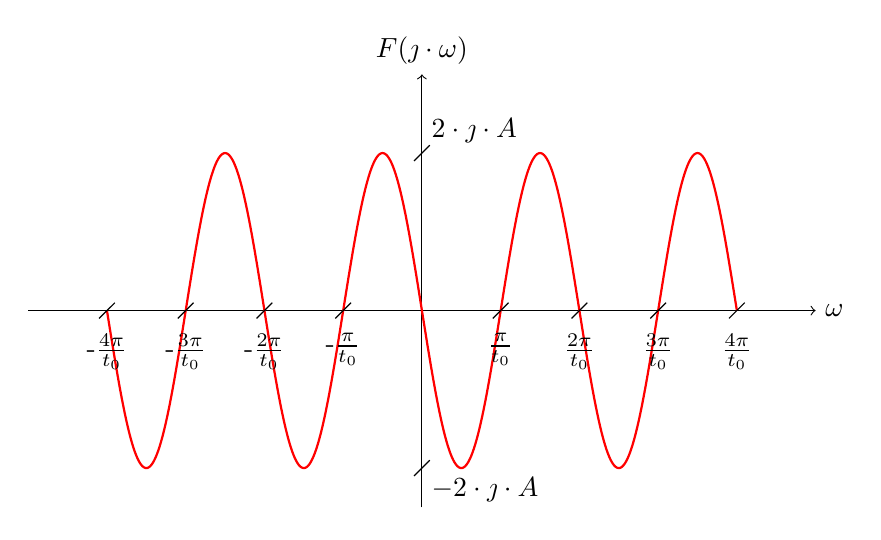
\begin{tikzpicture}
	\draw[->] (-5.0,+0.0) -- (+5.0,+0.0) node[right] {$\omega$};
	\draw[->] (+0.0,-2.5) -- (+0.0,+3.0) node[above] {$F(\jmath \cdot \omega)$};

	\draw[scale=1.0,domain=-4.0:4.0,samples=2000,smooth,variable=\x,red,thick] plot ({\x},{-2*sin(\x*180)});

	\draw[-] (-1.0-0.1,-0.1)--(-1.0+0.1,0.1) node[midway, below, outer sep=5pt] {-$\frac{\pi}{t_0}$};
	\draw[-] (-2.0-0.1,-0.1)--(-2.0+0.1,0.1) node[midway, below, outer sep=5pt] {-$\frac{2 \pi}{t_0}$};
	\draw[-] (-3.0-0.1,-0.1)--(-3.0+0.1,0.1) node[midway, below, outer sep=5pt] {-$\frac{3 \pi}{t_0}$};
	\draw[-] (-4.0-0.1,-0.1)--(-4.0+0.1,0.1) node[midway, below, outer sep=5pt] {-$\frac{4 \pi}{t_0}$};
	\draw[-] (+1.0-0.1,-0.1)--(+1.0+0.1,0.1) node[midway, below, outer sep=5pt] {$\frac{\pi}{t_0}$};
	\draw[-] (+2.0-0.1,-0.1)--(+2.0+0.1,0.1) node[midway, below, outer sep=5pt] {$\frac{2 \pi}{t_0}$};
	\draw[-] (+3.0-0.1,-0.1)--(+3.0+0.1,0.1) node[midway, below, outer sep=5pt] {$\frac{3 \pi}{t_0}$};
	\draw[-] (+4.0-0.1,-0.1)--(+4.0+0.1,0.1) node[midway, below, outer sep=5pt] {$\frac{4 \pi}{t_0}$};
	\draw[-] (-0.1,+2.0-0.1)--(+0.1,+2.0+0.1) node[midway, above right] {$2 \cdot \jmath \cdot A$};
  \draw[-] (-0.1,-2.0-0.1)--(+0.1,-2.0+0.1) node[midway, below right] {$-2 \cdot \jmath \cdot A$};

	\end{tikzpicture}
\end{figure}

\TT{Widmo amplitudowe obliczamy ze wzoru:}{The magnitude spectrum is defined as:}

\begin{align*}
M(\omega)&=\left | F(j \cdot \omega) \right |\\
&=\sqrt{\left(-2 \cdot A \cdot sin(\omega \cdot t_0)\right)^2}\\
&=\sqrt{4 \cdot A^2 \cdot sin^2(\omega \cdot t_0)}\\
&=2 \cdot A \cdot \left | sin(\omega \cdot t_0) \right |
\end{align*}

\begin{figure}[H]
	\centering
	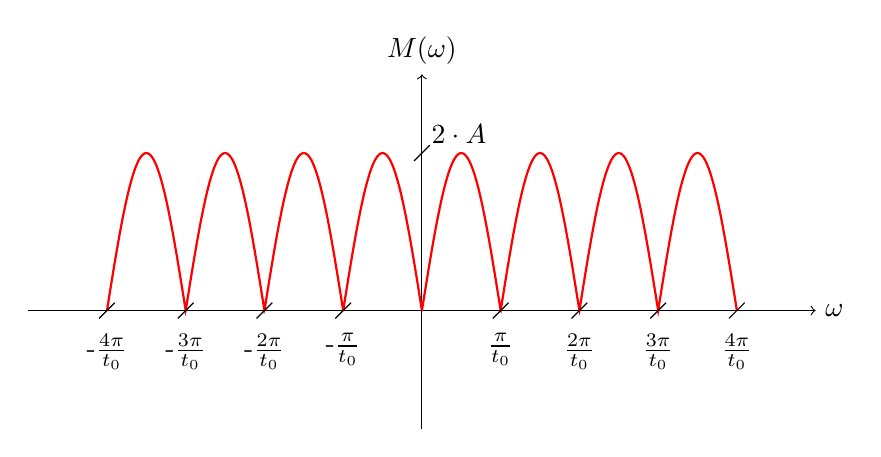
\begin{tikzpicture}
	\draw[->] (-5.0,+0.0) -- (+5.0,+0.0) node[right] {$\omega$};
  \draw[->] (+0.0,-1.5) -- (+0.0,+3.0) node[above] {$M(\omega)$};
  
  \draw[scale=1.0,domain=-4.0:4.0,samples=2000,smooth,variable=\x,red,thick] plot ({\x},{abs(-2*sin(\x*180))});
  
  \draw[-] (-1.0-0.1,-0.1)--(-1.0+0.1,0.1) node[midway, below, outer sep=5pt] {-$\frac{\pi}{t_0}$};
  \draw[-] (-2.0-0.1,-0.1)--(-2.0+0.1,0.1) node[midway, below, outer sep=5pt] {-$\frac{2 \pi}{t_0}$};
  \draw[-] (-3.0-0.1,-0.1)--(-3.0+0.1,0.1) node[midway, below, outer sep=5pt] {-$\frac{3 \pi}{t_0}$};
  \draw[-] (-4.0-0.1,-0.1)--(-4.0+0.1,0.1) node[midway, below, outer sep=5pt] {-$\frac{4 \pi}{t_0}$};
  \draw[-] (+1.0-0.1,-0.1)--(+1.0+0.1,0.1) node[midway, below, outer sep=5pt] {$\frac{\pi}{t_0}$};
  \draw[-] (+2.0-0.1,-0.1)--(+2.0+0.1,0.1) node[midway, below, outer sep=5pt] {$\frac{2 \pi}{t_0}$};
  \draw[-] (+3.0-0.1,-0.1)--(+3.0+0.1,0.1) node[midway, below, outer sep=5pt] {$\frac{3 \pi}{t_0}$};
  \draw[-] (+4.0-0.1,-0.1)--(+4.0+0.1,0.1) node[midway, below, outer sep=5pt] {$\frac{4 \pi}{t_0}$};
  \draw[-] (-0.1,+2.0-0.1)--(+0.1,+2.0+0.1) node[midway, above right] {$2 \cdot A$};
  		
	\end{tikzpicture}
\end{figure}

\TT{Widmo fazowe obliczamy ze wzoru:}{The phase spectrum is defined as:}

\begin{equation}
\Phi ( \omega )=\TT{arctg}{arctan2}\left(\frac{Im\{F(\jmath \cdot \omega )\}}{Re\{F(\jmath \cdot \omega )\}}\right)
\end{equation}

\begin{figure}[H]
	\centering
	\begin{tikzpicture}
	\draw[->] (-5.0,+0.0) -- (+5.0,+0.0) node[right] {$\omega$};
	\draw[->] (+0.0,-1.5) -- (+0.0,+2.0) node[above] {$\Phi(\omega)$};
	
	\draw[-,red] (-4.0,-1.0) -- (-3.0,-1.0);
	\draw[-,red] (-3.0,+1.0) -- (-2.0,+1.0);
	\draw[-,red] (-2.0,-1.0) -- (-1.0,-1.0);
	\draw[-,red] (-1.0,+1.0) -- (0.0,+1.0);
	\draw[-,red] (0.0,-1.0) -- (1.0,-1.0);
	\draw[-,red] (1.0,+1.0) -- (2.0,+1.0);
	\draw[-,red] (2.0,-1.0) -- (3.0,-1.0);
 	\draw[-,red] (3.0,+1.0) -- (4.0,+1.0);
	  
	\draw[-] (-1.0-0.1,-0.1)--(-1.0+0.1,0.1) node[midway, below, outer sep=5pt] {-$\frac{\pi}{t_0}$};
	\draw[-] (-2.0-0.1,-0.1)--(-2.0+0.1,0.1) node[midway, below, outer sep=5pt] {-$\frac{2 \pi}{t_0}$};
	\draw[-] (-3.0-0.1,-0.1)--(-3.0+0.1,0.1) node[midway, below, outer sep=5pt] {-$\frac{3 \pi}{t_0}$};
	\draw[-] (-4.0-0.1,-0.1)--(-4.0+0.1,0.1) node[midway, below, outer sep=5pt] {-$\frac{4 \pi}{t_0}$};
	\draw[-] (+1.0-0.1,-0.1)--(+1.0+0.1,0.1) node[midway, below, outer sep=5pt] {$\frac{\pi}{t_0}$};
	\draw[-] (+2.0-0.1,-0.1)--(+2.0+0.1,0.1) node[midway, below, outer sep=5pt] {$\frac{2 \pi}{t_0}$};
	\draw[-] (+3.0-0.1,-0.1)--(+3.0+0.1,0.1) node[midway, below, outer sep=5pt] {$\frac{3 \pi}{t_0}$};
	\draw[-] (+4.0-0.1,-0.1)--(+4.0+0.1,0.1) node[midway, below, outer sep=5pt] {$\frac{4 \pi}{t_0}$};
	\draw[-] (-0.1,+1.0-0.1)--(+0.1,+1.0+0.1) node[midway, above left] {$\frac{\pi}{2}$};
	\draw[-] (-0.1,-1.0-0.1)--(+0.1,-1.0+0.1) node[midway, left] {-$\frac{\pi}{2}$};
	
	\end{tikzpicture}
\end{figure}

\end{task}

